%
\documentclass[10pt, conference, compsocconf]{IEEEtran}
\usepackage[ruled,vlined]{algorithm2e}
\usepackage{algpseudocode}
\usepackage[utf8]{inputenc}
\usepackage{tabularx}
\usepackage{amsmath}
\usepackage{graphicx}
\usepackage{float}

\begin{document}
\onecolumn
%
% paper title
% can use linebreaks \\ within to get better formatting as desired
\title{A Weighted Frequent Mining For Predicting Water Level In Winnipeg}


% author names and affiliations
% use a multiple column layout for up to two different
% affiliations

\author{\IEEEauthorblockN{Adam Bouttell, Sijin Lee, Martin Levesque, Seunggon Son, Weihong Zhang}
\IEEEauthorblockA{COMP 4710, Group 8\\
University of Manitoba\\
Winnipeg, Canada\\
Email: bouttela@myumanitoba.ca, lees3436@myumanitoba.ca, levesqum@myumanitoba.ca, \\
sons@myumanitoba.ca, zhangw22@myumanitoba.ca}
}


% make the title area
\maketitle


\begin{abstract}
In Winnipeg, water levels can be an indicator that affects the activities we do near the rivers/lakes. Water levels can also indicate potential disasters that are occurring. In this paper, we use three different categories of weather data collected from public sources as well as water levels collected from the red river near the Forks to generate model used for prediction. We evaluate three weighted frequency evaluation methods for prediction and evaluate its feasibility in terms of its accuracy in hopes to produce a model that can help people plan activities or avoid disasters. 

\end{abstract}

% For peer review papers, you can put extra information on the cover
% page as needed:
% \ifCLASSOPTIONpeerreview
% \begin{center} \bfseries EDICS Category: 3-BBND \end{center}
% \fi
%
% For peerreview papers, this IEEEtran command inserts a page break and
% creates the second title. It will be ignored for other modes.
\IEEEpeerreviewmaketitle

\section{Introduction}
% no \IEEEPARstart
In Winnipeg, water levels can be an indicator that affects the activities we do near the rivers/lakes. Water levels can also indicate potential disasters that are occurring. In this paper, we first gather the weather data from the Canadian government climate database and the water level from the Canadian Government water level database. We notice that the data collected are non-categorical, so we will then split the data into categories after some considerations that will be discussed in more detail in the next section.  After the data has been prepared, the data is split into training data and testing data. Then we evaluate the data in different ways and extract the weight from each process to generate different models used to predict the water level. In the end, we evaluate the predicted results and evaluates its feasibility. 

\section{Data Classification}
In order to easily scan data and to assign weight values to the data, it was necessary to group the data into labeled categories (Sampath et al.[1]). Once the data has been categorized, we can attach varying weights to different categories of data and then extract useful patterns from the data.

\medskip
\subsection{Rainfall}
\begin{center}
\begin{tabularx}{0.8\textwidth} { 
  | >{\centering\arraybackslash}X 
  | >{\centering\arraybackslash}X 
  |
  }
 \hline
 \textbf{Rainfall(mm)} & \textbf{Categorized Rainfall} \\
 \hline
0  & No Rain  \\
\hline
0.1 - 9  & Drizzle \\
\hline
 10 - 19  & Light Rain \\
\hline
20 - 29 & Moderate Rain  \\
\hline
30 - 39  & Heavy Rain  \\
\hline
over 40   & Violent Rain  \\
\hline
\end{tabularx}
\end{center}
\medskip
For rain fall classification, there were six different groups indicating the intensity of rain fall (Sieck et al.[2]). 0 millimeters value was assigned to ‘No Rain’ which was the most frequent group and the rain fall values from 0.1 to 9 millimeters were grouped together into ‘Drizzle’ and this category appeared the second most frequent group. From 10 to 39 millimeters were split into three groups  and assigned to ’Light Rain’, ‘Moderate Rain’ and ‘Heavy Rain’ in 10 millimeters intervals respectively as the value increases. All values captured as over 40 millimeters were categorized into ‘Violent Rain’ (Goodison et al.[3]).
\medskip
\subsection{Wind}
\begin{center}
\begin{tabularx}{0.8\textwidth} { 
  | >{\centering\arraybackslash}X 
  | >{\centering\arraybackslash}X 
  |
  }
 \hline
 \textbf{Wind(km/h)} & \textbf{Categorized Wind} \\
 \hline
less than 32 & Low  \\
\hline
32 - 44  & Moderate \\
\hline
45 - 57 & Moderately High \\
\hline
58 - 70 & High  \\
\hline
over 71 & Extreme  \\
\hline
\end{tabularx}
\end{center}
\medskip
For wind speed, all values under 32 kilometers per hour were grouped together and all higher wind speeds were separated into evenly spaced intervals. This method of grouping results in low wind speeds being the most common group, while other categories of wind speeds occur with decreasing frequency the higher the wind speed becomes.
\medskip
\subsection{Temperature}
\begin{center}
\begin{tabularx}{0.8\textwidth} { 
  | >{\centering\arraybackslash}X 
  | >{\centering\arraybackslash}X 
  |
  }
 \hline
 \textbf{Temperature(°C)} & \textbf{Categorized Temperature} \\
 \hline
 -29 - -20 & Extreme Cold \\
\hline
-19 - -10 & Very Cold \\
\hline
-9 - 0 & Cold \\
\hline
1 - 10 & Neutral  \\
\hline
11 - 20 & Warm  \\
\hline
21 - 30 & Hot  \\
\hline
31 - 40 & Very Hot \\
\hline
\end{tabularx}
\end{center}
\medskip
  For temperature classification, due to the absence of data below -29 °C and over 40 °C, the temperature range between -29°C to 40°C was only considered to be categorized. All values were separated into seven different groups in 10°C interval from -29 °C, to 40 °C (Peel et al.[4]). 
  \medskip
\subsection{Water Level}
\begin{center}
\begin{tabularx}{0.8\textwidth} { 
  | >{\centering\arraybackslash}X 
  | >{\centering\arraybackslash}X 
  |
  }
 \hline
 \textbf{Water Level(m)} & \textbf{Categorized Water Level} \\
 \hline
222.000- 222.999 &  Low \\
\hline
223.000 - 223.999 & Moderate \\
\hline
224.000 -224.999 & Moderately High \\
\hline
225.000 -225.999 & High  \\
\hline
over 226 & Very High  \\
\hline
\end{tabularx} 
\end{center}
\medskip
  For water level classification, five different groups were made and each group were separated based on 1 meter interval from the water level of 222.000 meter except for the water level over 226.000 meter. This allows us to give weight values to each category to give importance to either high or low values when we are mining the data.
\medskip
\medskip

\section{Categorical Testing}
\subsection{Introduction}
The weight is generated by the frequent water level that appears in one category. Each category would 
be combined with other categories in other classification such as 'no rain' of rainfall with 'extreme cold' of temperature and then it will be one pair to predict water level. It means that a weight value would be summed with other categories' weights. Then, we can get a maximum weight value for comparing with the testing model. 
For example, in the rainfall classification, there are \{No Rain, Drizzle, ...\} and in the temperature classification, there are \{Extreme Cold, Cold, ...\}. Each category has own weight values for each water level. If we would like to predict water level when \{NO Rain\} and \{Extreme Cold\}, then sum every weight value at the same water level. Then, we can get an expected water level by a maximum weight value. Finally, The expected water level should be compared with testing data in the same environment. 


\subsection{Training Step}
To generate weight values, collect frequents of each water level for categories. Each category is divided into water levels. For example, there is a total of 395 data of the 'no rain' in the rainfall classification, and there are 181 of 'Low' and 134 of 'Moderate' in the water level category. So, in order to generate the weight values of 'No Rain' in low water level, we have to get the support values of the 'No Rain', and get water level support values from the 'No Rain' category.
\begin{equation*}
weight = \frac{sup({Cat}_{WL})}{sup({Cat})}
\end{equation*}
where Cat = category of the classification
WL = Water level from the category

\subsection{Testing step}
We can get the expected water level in a specific environment in the training data. Using these expected data, we can start to predict the water level. We create a training model using the 2014 \& 2015 data and test model using 2016 data, so we can compare the expected water level in the training model and actual water level in the test model in the same environment. 

\begin{equation*}
\{SumOfWeight\}=\{{WeightRain}_{WL}\}+\{{WeightTemp}_{WL}\}+\{{WeightWind}_{WL}\}
\end{equation*}

\begin{algorithm}
\SetAlgoLined
\KwResult{Calculate Prediction Calculation}
    initialization\;
    ActWL = Actual Water Level\;
    ExpWL = Water level of maximum weight\;
    CorrectPredict = 0\;
    \For{all predicted data points}{
        \uIf{ExpWL == ActWL}{
        CorrectPredict += 1\;
       }
    }
    Accuracy = CorrectPredict/TotalPredict
 \caption{Predicting Water Levels}
\end{algorithm}

\subsection{Result}
After the testing step, we can get this model's accuracy of 163/355, which is approximately 46\%. Furthermore, it matches only 'Low' and 'Moderate', which is respectively 76 for 'Low' and 86 for 'Moderate' out of 163. Therefore, this is not an accurate model for predicting the water level. In order to confirm the info in further detail, the binary classification was used. In the binary classification, it showed low result values. First result shows precision, recall, F1 and AUC values for each water level. The 'Low' class label showed higher accuracy scores than other classes, but the other classes are at 0.5 or a little higher. The values can be found in the following table.
\begin{center}
 \begin{tabular}{||c c c c c||} 
 \hline
 Water Level & Precision & Recall & F1 Score & ROC-AUC \\ [0.5ex] 
 \hline\hline
 Low & 0.385786 & 1.0 & 0.556776 & 0.783154 \\ 
 \hline
 Moderate & 0.550632 & 0.491525 & 0.519402 & 0.546324 \\
 \hline
 Moderately High & 0 & 0 & 0 & 0.5 \\
 \hline
 High & 0 & 0 & 0 & 0.5 \\
 \hline
 Very High & 0 & 0 & 0 & 0.5 \\ [1ex] 
 \hline
\end{tabular}
\end{center}

Secondly, we gathered all the data to figure out the accuracy of overall data. It also shows low result value that is close to 0.5. The values can be found in the following table and graph.
\begin{center}
 \begin{tabular}{||c c c c c||} 
 \hline
  & Precision & Recall & F1 Score & ROC-AUC \\ [0.5ex] 
 \hline\hline
 Macro & 0.187283 & 0.298305 & 0.215235 & 0.565895 \\ 
 \hline
\end{tabular}
\end{center}
\clearpage
\begin{figure}[H]
\begin{center}
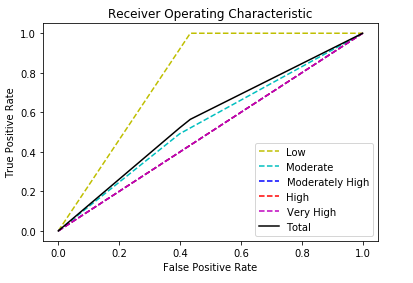
\includegraphics[width=0.9\linewidth]{vert_ROC.png}
\end{center}
\end{figure}
As a result, the above data showed that there is other classification to predict water level.

\section{Prediction Using Support Value Ratios}

\subsection{Introduction}

This second prediction model proposed in our project works by first generating a set of “weights” from the pre-processed training data with classified attributes. Weight values are assigned to each predictive attribute class – water level class pair (e.g. Low Wind – Moderate Water Level, Warm Temperature – High Water Level) by calculating the ratio of the support value of the “pair itemset” and the support value of the water level class of that pair. These weights are then used later to make predictions of the water level classifications based on the greatest “sum of weights” of the predictive attributes (namely rainfall, temperature, and wind).

\subsection{Training the Prediction Model}

To generate the weights used by the prediction model, we first iterate over each possible water level class and query the training data set to attain all the records that contain the current water level class being examined. The number of records that are returned gives us the support value for the water level class in question which will be used as the denominator of all ratio calculations for this current class. Once we are returned the list of records that contain the water level class used in the current iteration, we then iterate through each possible predictive attribute class and query the result of the first query for records that contain the current predictive attribute class. The count of records returned from this secondary query is then used as the numerator for the ratio calculation for the current predictive attribute class – water level class pair. Once we calculate the ratio value for the current “class pair”, we store the result and continue iterating through each predictive attribute class to find the ratio values for subsequent class pairs, then repeat this process for each water level class. To summarize, the calculation of the weight for each predictive attribute class – water level class pair is as follows:

\begin{equation*}
{Weight}_{(WL, PA)}=\frac{\sup{\left(\left\{WL,\ PA\right\}\right)}}{sup(\left\{WL\right\})}
\end{equation*}
\noindent
where WL = current water level class, PA = current predictive attribute class, and Weight\textsubscript{(WL, PA)} = generated weight for the current “water level class – predictive attribute class” pair.

\subsection{Making Predictions with the Trained Model}

Once all possible class pairs have been assigned a weight value using the training data set, the prediction model is now ready to start making predictions on the records from our testing data set. To make a prediction for a given set of predictive attributes (rainfall level class, temperature level class, and wind level class), the model will index the set of weights generated from the training step using the provided predictive attribute classes to generate the “sum of weights” for each possible water level class. The calculation of this “sum of weights” for a given water level class is as follows:

\begin{equation*}
\begin{split}
{SumOfWeights}_{(WL)}={Weight}_{(WL, RainL)}+\\ {Weight}_{(WL, TempL)}+&{Weight}_{(WL, WindL)}
\end{split}
\end{equation*}
\noindent
where WL = water level class, RainL = rainfall level class, TempL = temperature level class, and WindL = wind level class. The water level class that gives the largest weight sum value with the provided set of predictive attributes is chosen by our model as the prediction.

\subsection{Results}

After training this model on the compiled 2014-2015 data and testing the model against the 2016 data, we found the following macro-averaged accuracy scores for the overall accuracy of the model:

\begin{center}
\begin{tabular}{ |c|c|c|c| } 
 \hline
 Precision & Recall & F1 Score & ROC-AUC Score \\ 
 \hline
 0.301389595 & 0.302066607 & 0.283481458 & 0.568085347 \\
 \hline
\end{tabular}
\end{center}

Looking at these results in more detail by considering the accuracy of predicting specific water levels, we found that the "Low" and "Moderately High" class labels had much higher accuracy scores when compared to other class labels. The following table and graph illustrates the skewed nature of the prediction model's accuracy:

\begin{figure}[ht]
\begin{center}
\begin{tabular}{ |c|c|c|c|c| } 
 \hline
 Water Level & Precision & Recall & F1 Score & ROC-AUC \\ 
 \hline
 Low & 0.563106796 & 0.763157895 & 0.648044693 & 0.800933786 \\
 \hline
 Moderate & 0.453125 & 0.163841808 & 0.2406639 & 0.483606297 \\
 \hline
 Moderately High & 0.413793103 & 0.45 & 0.431137725 & 0.632272727 \\ 
 \hline
 High & 0.076923077 & 0.133333333 & 0.097560976 & 0.531372549 \\ 
 \hline
 Very High & 0 & 0 & 0 & 0.392241379 \\ 
 \hline
\end{tabular}
\end{center}
\includegraphics[width=0.9\linewidth]{"Model Accuracy Graph - Cropped".pdf}
\centering
\end{figure}

The effectiveness of this prediction model can also be illustrated with the help of Receiver Operating Characteristic (ROC) curves. The following graph plots the ROC curves for each water level class as well as the macro-averaged ROC curve that gives a measure for the overall accuracy of the model:

\begin{figure}[ht]
\includegraphics[width=1\linewidth]{"ROC Curves".png}
\centering
\caption{ROC Curves for Specific Water Levels}
\end{figure}

We can attribute the skewed accuracy seen in our results to the relatively small size of our training data set (only 689 records) and the unequal distribution of water levels within our training data. The majority of the records within our training data set have water levels that are on the lower end of the range of possible values. This skewed distribution within our training data likely contributed to the higher accuracy of our model correctly predicting lower water levels. The small size of our training data also likely contributed to the skewed accuracy by not allowing the prediction model to observe a wide range of possible scenarios. If we were able to find larger sets of historical data, we would likely have more accurate/useful weight values that would give our model a better chance at making correct predictions.

\section{Prediction Using Frequent Data-sets with Relative Weights}

\subsection{Introduction}

One approach that we tried when generating predictions of classified water levels was to first extract the frequent data-sets from the training data-set. This is based off the basic form of the Apriori algorithm used for data mining.Then we introduce weights to the categories collected similar to the method introduced by (Yun and Leggett[5]).

\subsection{Data Collection Step}

We do this by collecting all the categories that are deemed to be frequent; and a category was considered frequent if the weight in the water level specification exceeds 10\%. For example, in the 302 data points of the training data-set that has “CategorizedWaterLevel” classified as “Low”, there are 181 data points that have “No Rain” and 118 data points that have “Drizzle” in the “CategorizedRainLevel”. These data points are considered frequent for “Low” water levels. We will be only looking at the single data frequency of the dataset as classifying minimum support as 10\% already excludes a high amount of categories. If we do investigate further into the combinations of categories and setting a minimum support on the combinations, there will be too few categories to use for predictions.
This method will be used to extract all the frequent categories for each water level in the training data set. Again, an example of this would be listed below:\\
\\
Low Water Level\\
Categorized Rain Level: No Rain, Drizzle\\
Categorized Temperature: Extreme Cold, Very Cold, Cold, Neutral\\
Categorized Wind Level: Low, Moderate\\
\\
With the categories selected, we will be looking at every combination of the three categories. So for low water level, such combinations can be \{No Rain, Extreme Cold, Low\}, \{Drizzle, Very Cold, Low\}, etc. 

\subsection{Prediction Step}
For explanation purposes, the combinations listed above are only exclusively frequent for low water level. If the data points in the three categories in the testing data are \{No Rain, Extreme Cold, Low\}, then the prediction for the water level will be “Low”. Now if there are overlapping categories in the data set, we will generate a weight for the overlapping categories with regard to the number of occurrences in each water level category. So consider the combination \{No Rain, Neutral, Low\}, this combination is frequent in Low Water Level, Moderate Water Level, Moderately High Water Level, and Very High Water Level. So we will consider the amount of times this combination appears in each water level divided by its total appearance to be the weight of the prediction for each of the water levels. Then a random number between 0-1 is generated to determine the actual prediction for a data point with this particular combination. The pseudo-code for the algorithm will be displayed in Algorithm 1.

\begin{algorithm}
\SetAlgoLined
\KwResult{generate a water level based on input category}
    initialization\;
  \eIf{If combination is unique to only one water level}{
    Predict the data to be of this water level\;
   }{
    Get total number of occurrence of this combination.(Total Weight)\;
    Get Weight for each particular water level (e.g. # of occurrence in water level1/Total Weight = W1)\;
	Generate random number\;
	\uIf{random number < W1}{
	    predict water level 1(e.g. Low)\;
	}
	\uIf{random number between W1, W1+W2}{
	   predict water level 2 (e.g. moderate)\;
	}
    ...\;
  }
 \caption{Predicting Water Levels}
\end{algorithm}

\subsection{Result}
We ran this algorithm on 10 seeds for the random number generation, and took the average of the number of correct predictions as a result of using this algorithm. Overall, this prediction method has an average accuracy of 134/355, which is 38\%. Now there is also a slight problem of infrequent combinations showing up and the algorithm not predicting for those combinations. For our testing data, there are 29 such cases where no predictions are made. We will assign the cases with a "Low" prediction as it is the most frequent occurring data in the training data set. A breakdown of the random seed prediction accuracy is shown in figure 2.

\begin{figure}[H]
\includegraphics[width=0.7\linewidth]{"Accuracy".png}
\centering
\caption{Precision of prediction for using different seeds to predict water levels}
\end{figure}

The following is the overall accuracy measurement of the data set:\\

\begin{center}
\begin{tabular}{ |c|c|c|c| } 
 \hline
 Precision & Recall & F1 Score & ROC-AUC Score \\ 
 \hline
 0.307146520 & 0.317218258 & 0.266835085 & 0.5805188796 \\
 \hline
\end{tabular}
\end{center}

We can breakdown the data further into the accuracy measure for each water level:\\

\begin{center}
\begin{tabular}{ |c|c|c|c|c| } 
 \hline
 Water Level & Precision & Recall & F1 Score & ROC-AUC \\ 
 \hline
 Low & 0.417142857 & 0.960526315 &  0.581673306 & 0.797467458 \\
 \hline
 Moderate & 0.625 & 0.367231638 & 0.462633451 & 0.574065257 \\
 \hline
 Moderately High & 0.41666666 & 0.125 & 0.1923076923 & 0.537045454 \\ 
 \hline
 High & 0.076923077 & 0.133333333 & 0.097560976 & 0.531372549 \\ 
 \hline
 Very High & 0 & 0 & 0 & 0.4626436781 \\ 
 \hline
\end{tabular}
\end{center}\\

Again, the effectiveness of this prediction model can be illustrated by Receiver Operating Characteristic (ROC) curves. The following graph plots the ROC curves for each water level class as well as the macro-averaged ROC curve that gives a measure for the overall accuracy of the model:

\begin{figure}[H]
\includegraphics[width=1\linewidth]{"Relative Weights ROC Curves".png}
\centering
\caption{ROC Curves for Specific Water Levels using Relative Weights}
\end{figure}

Overall, this approach is infeasible based on the data structure that we have set up due to the data being skewed more to the low and moderate water levels. 

\section{Conclusion}
With the three models generated from different methods of classifying data, we can see the first two methods rely heavily on the data being more skewed to particular categories for it to generate an accurate prediction, as for the frequent data sets method, it is difficult to classify data with limited amount of explanatory variables as it can't gather enough frequent categories to generate proper predictions. One way all the algorithms can be improved is with finding more relevant explanatory variables to expand the model building process. Overall, the three models generated are not feasible to predict water levels as of yet. It can be improved further in the future as more data is collected.

\begin{thebibliography}{1}

\bibitem{IEEEhowto:kopka}K. K. Sampath and P. K. Karthik, “Determining frequent itemsets using partitioning technique for large transaction database,” Indian Journal of Science and Technology , vol. 12, no. 3, pp. 1–4, 2019.\\

\bibitem{IEEEhowto:kopka}Sieck, L.C., S.J. Burges and M. Steiner, 2007: Challenges in obtaining reliable measurements of point rainfall. Water Resources Research, 43:1–23. \\

\bibitem{IEEEhowto:kopka}WMO Solid Precipitation Measurement Intercomparison: Final Report (B.E. Goodison, P.Y.T. Louie and D. Yang). Instruments and Observing Methods Report No. 67 (WMO/TD-No. 872). Geneva. \\

\bibitem{IEEEhowto:kopka}Peel, M. C., Finlayson, B. L., and McMahon, T. A.: Updated world map of the Köppen-Geiger climate classification, Hydrol. Earth Syst. Sci., 11, 1633–1644, https://doi.org/10.5194/hess-11-1633-2007, 2007.\\

\bibitem{IEEEhowto:kopka}
Yun U, Leggett J (2005) Wfim: weighted frequent itemset mining with a weight range and a minimum weight. In: Proceeding of the 2005 SIAM international conference on data mining (SDM’05), Newport Beach, CA, pp 636–640

\end{thebibliography}




% that's all folks
\end{document}
